\documentclass{article}
\usepackage[utf8]{inputenc}

\usepackage{geometry}
\usepackage{bm}
\geometry{a4paper}
\usepackage{latexsym}
%\usepackage[dvips]{graphicx}
\usepackage{epsfig}
\usepackage{amsmath}
\usepackage{amsfonts}
\usepackage{amssymb}
\usepackage{eucal}
\usepackage{mathrsfs}
\usepackage{wasysym}
\usepackage{setspace}
\usepackage{float}
\usepackage{color}
\usepackage{rotating}
\usepackage{stmaryrd}
\usepackage{lineno}

\numberwithin{equation}{section}
\frenchspacing
%%
\usepackage{amsthm}


%%%%INSERITI ADESSO%%%%
\usepackage{amsmath}
\usepackage{amsfonts}
\usepackage{amssymb}
\usepackage{amsthm}
\usepackage{mathrsfs}
\usepackage{eucal}  
\theoremstyle{definition}
\usepackage{accents}
\usepackage{array}
\usepackage{cases}
\usepackage{graphicx}
\usepackage{booktabs}
\usepackage{caption}
\usepackage{cancel}
\usepackage{bbm}
\usepackage{subfig}
\usepackage{enumitem}
\usepackage{movie15}
 \usepackage{algorithm}
\usepackage{algpseudocode}
\usepackage{tabularx}
\usepackage{longtable}
 
% Font Management
\usepackage[T1]{fontenc}       % 8 bit font encoding: includes all accents
\usepackage{bm}                % alternative to \bs provided by package amsmath
\usepackage{bbm}               % alternative to \mathbb;  usage: \mathbbm{}
%\usepackage[mathscr]{eucal}    % alternative to \mathcal; usage: \mathcal{}
\usepackage{color}             % for text in colour
\usepackage{verbatim}          % environment for commenting out blocks of text
%\usepackage{exscale}           % needed to scale cmdx fonts
%\usepackage{ae,aecompl}        % see http://www.ctan.org/tex-archive/fonts/ae
%%%%%%%%%%%%%%%%%%


\theoremstyle{plain}
\newtheorem{thm}{Teorema}[section]
\newtheorem{lem}[thm]{Lemma}
\newtheorem{prop}[thm]{Proposizione}
\newtheorem*{cor}{Corollario}

\theoremstyle{definition}
\newtheorem{defn}{Definizione}[section]
\newtheorem{conj}{Congettura}[section]
\newtheorem{exmp}{Esempio}[section]

\theoremstyle{remark}
\newtheorem*{rem}{Osservazione}
\newtheorem*{note}{Nota}

\DeclareMathOperator*{\argmin}{argmin}
\DeclareMathOperator*{\argmax}{argmax}

\newcommand{\dom}{\mathrm{dom}}
\newcommand{\im}{\mathrm{im}}
\newcommand{\sign}{\mathrm{sign}}
\newcommand{\abs}{\mathrm{abs}}
\newcommand{\e}{\mathrm{exp}}

\setlength{\textwidth}{15 cm}
\setlength{\textheight}{23.5 cm}



%%%%%%%%%%%%%%%%%%%%%%%%%%%%%%%%%%%%%%%%%%%%%%%%%%%

\usepackage[utf8]{inputenc}
\usepackage[T1]{fontenc}
\usepackage{lmodern}

\usepackage{hyperref}
\hypersetup{%
    pdfpagemode={UseOutlines},
    bookmarksopen,
    pdfstartview={FitH},
    colorlinks,
    linkcolor={blue},
    citecolor={blue},
    urlcolor={blue}
  }

%%%%%%% use PDFLATEX 

\usepackage{lipsum} %to insert random text

\usepackage{geometry} %for the margins
\newcommand\fillin[1][4cm]{\makebox[#1]{\dotfill}} %for the dotted line in the frontispiace

\usepackage{dcolumn}
\newcolumntype{d}{D{.}{.}{-1} } %to vetical align numbers in tables, along the decimal dot

\usepackage{amsmath}



%%%%%%% Local definitions
\newtheorem{osservazione}{Osservazione}% Standard LaTeX
\newtheorem{observation}{Observation}% Standard LaTeX

\newcommand{\BR}{\mathscr{B}_{\mathrm{R}}}
\newcommand{\T}[2]{T_{#2}#1}
\newcommand{\cT}[2]{T_{#2}^{*}#1}
\newcommand{\pder}[2]{\frac{\partial #1}{\partial #2}}

				 
%%%%%%%%%%%%%%%%%%%%%%%%%%%%%%%%%%%%%%%%%%%%%%%%%
%
% Inserito il codice Matlab
%
\usepackage{listings}
\usepackage{hyperref}
\usepackage{xcolor}

\definecolor{codegreen}{rgb}{0,0.6,0}
\definecolor{codegray}{rgb}{0.5,0.5,0.5}
\definecolor{codepurple}{rgb}{0.58,0,0.82}
\definecolor{backcolour}{rgb}{0.95,0.95,0.92}

\lstdefinestyle{mystyle}{
    backgroundcolor=\color{backcolour},   
    commentstyle=\color{codegreen},
    keywordstyle=\color{magenta},
    numberstyle=\tiny\color{codegray},
    stringstyle=\color{codepurple},
    basicstyle=\ttfamily\footnotesize,
    breakatwhitespace=false,         
    breaklines=true,                 
    captionpos=b,                    
    keepspaces=true,                 
    numbers=left,                    
    numbersep=4pt,                  
    showspaces=false,                
    showstringspaces=false,
    showtabs=false,                  
    tabsize=2
}

\lstset{style=mystyle}


\title{Computational Linear Algegbra For Large Scale Problems}
\author{Nenna Giulio, Ornella Elena Grassi}
\date{Spectral Clustering Homework}
\begin{document}
\maketitle
The aim of this homework is to implement and apply \textbf{Spectral Clustering} to two different sets of datapoints in \(\mathbb{R}^2\). The two sets are shown in Figure \ref{scatter_intro}
\begin{figure}[H]
  \centering
  \subfloat[1][Scatterplot of the data stored in \texttt{Circle.mat}]{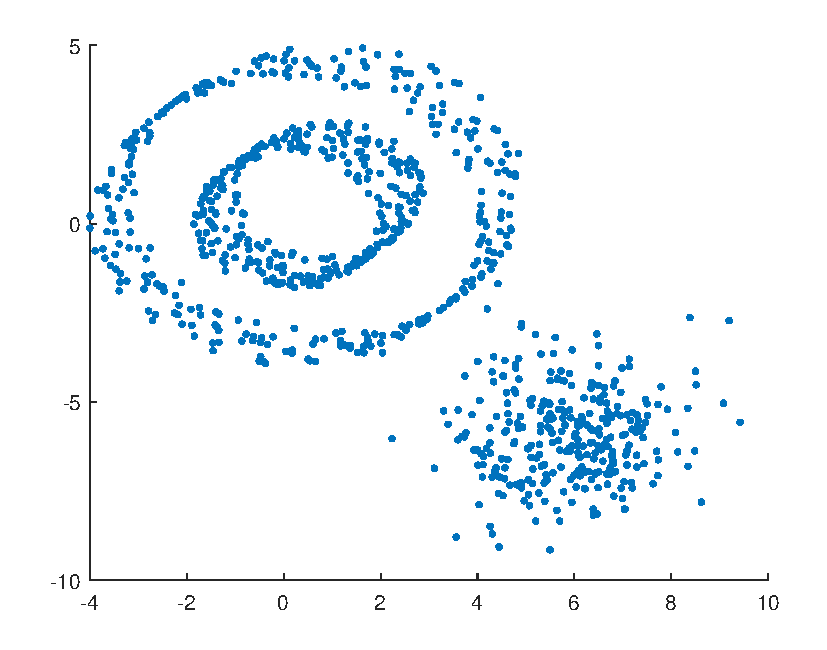
\includegraphics[scale = 0.45]{pictures/circle_scatterplot.pdf}}
  \qquad
  \qquad
  \subfloat[2][Scatterplot of the data stored in \texttt{Spiral.mat}]{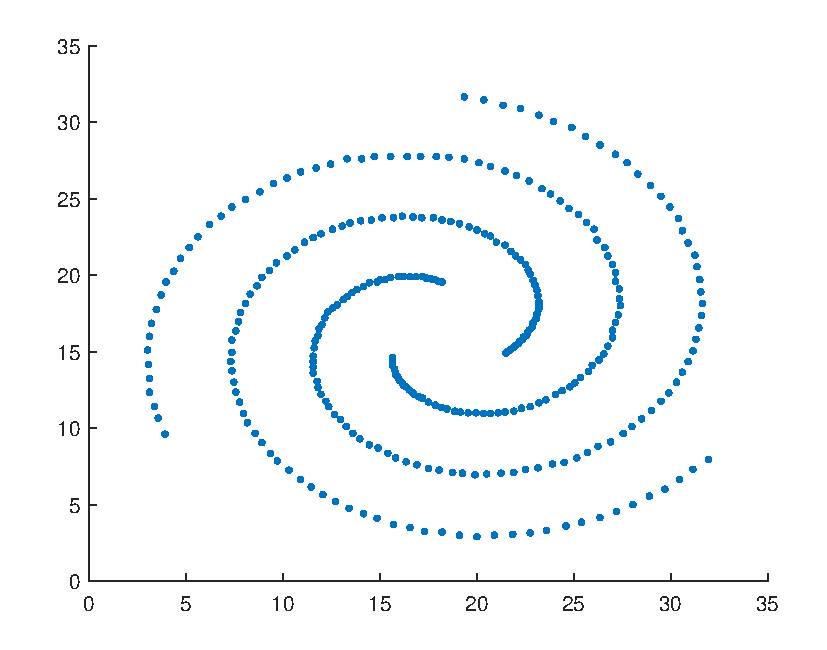
\includegraphics[scale = 0.45]{pictures/spiral_scatterplot.pdf}}
  \caption{Scatterplot of the two Datasets}
  \label{scatter_intro}
\end{figure}

As it is clearly visible through visual inspection, both datasets contain \(3\) different shapes that can be classified as different clusters. In the \texttt{Circle} dataset there are two concentrical circles and a cloud of points in the bottom right while in the \texttt{Spiral} dataset there are 3 spirals. Traditional clustering algorithms, that mainly rely on euclidean distance, may fail in recognizing the presence of shapes in our data hence our need to rely on a different technique called \textbf{Spectral clustering}. 
\\
\\

\section{K-Nearest Neighborhood Graph}
First, we need to define a similarity function that measures "how much our points are similar to each other". Let \(X_i\) and \(X_j\) be two points in our data, then we will use a similarity measure defined as:
\begin{equation}
  s_{i,j} = \exp \left(- \frac{\| X_i- X_j \|^2}{2\sigma^2}\right)
\end{equation}
Then, a \textit{\(K\)-Nearest Neighborhood} similarity graph is a Graph \(G= (V,E)\) where each vertex \(v_1, \dots v_n\) represents a point and two vertices \(v_i\) and \(v_j\) are connected by an undirected edge \(e_{i,j}\) if the similarity between \(v_i\) and \(v_j\) is among the \(K\)-th highest similarities between \(v_i\) and other vertices in \(V\). For such graph we can define the relative adjacency matrix as \(W_{i,j} = s_{i,j}\) where each entry \(W_{i,j}\) is nonzero only if there exists an edge between \(v_i\) and \(v_j\). \(W\) has zero-values on diagonal by definition.
\\
\\
The following MATLAB code was use to generate the K-NN similarity graph of our data:


%\bibliographystyle{plain} % We choose the "plain" reference style
%\bibliography{refs} % Entries are in the refs.bib file


\end{document}